% TEMPLATE for Usenix papers, specifically to meet requirements of
%  USENIX '05
% originally a template for producing IEEE-format articles using LaTeX.
%   written by Matthew Ward, CS Department, Worcester Polytechnic Institute.
% adapted by David Beazley for his excellent SWIG paper in Proceedings,
%   Tcl 96
% turned into a smartass generic template by De Clarke, with thanks to
%   both the above pioneers
% use at your own risk.  Complaints to /dev/null.
% make it two column with no page numbering, default is 10 point

% Munged by Fred Douglis <douglis@research.att.com> 10/97 to separate
% the .sty file from the LaTeX source template, so that people can
% more easily include the .sty file into an existing document.  Also
% changed to more closely follow the style guidelines as represented
% by the Word sample file. 

% Note that since 2010, USENIX does not require endnotes. If you want
% foot of page notes, don't include the endnotes package in the 
% usepackage command, below.

% This version uses the latex2e styles, not the very ancient 2.09 stuff.
\documentclass[letterpaper,twocolumn,10pt]{article}
\usepackage{usenix,epsfig,endnotes}
\usepackage{graphicx}
\usepackage{float}
% \newfloat{listing}{htbp}{scl}[section]
% \floatname{listing}{Listing}
\usepackage{minted}
\interfootnotelinepenalty=10000
\usepackage{lipsum}                     % Dummytext
\usepackage{xargs}                      % Use more than one optional parameter in a new commands
\usepackage[pdftex,dvipsnames]{xcolor}  % Coloured text etc.
% 
\usepackage[colorinlistoftodos,prependcaption,textsize=tiny]{todonotes}
\newcommandx{\comment}[2][1=]{\todo[linecolor=red,backgroundcolor=orange!25,bordercolor=red,inline,size=\small#1]{#2}}

% imports for hyper link 
\usepackage{hyperref}
\hypersetup{
    colorlinks=false,
    linkcolor=blue,
    filecolor=blue,      
    urlcolor=cyan,
}
% \hypersetup{
%     colorlinks=true,%MAKE FALSE BEFORE SUBMIT
%     linkcolor=blue,
%     filecolor=blue,      
%     urlcolor=cyan,
% }

% imports for code highlight
% \usepackage{listings, listings-rust}
\usepackage{xcolor}

\definecolor{dkgreen}{rgb}{0,0.6,0}
\definecolor{gray}{rgb}{0.5,0.5,0.5}
\definecolor{mauve}{rgb}{0.58,0,0.82}
\usepackage{csquotes}
\usepackage{dirtytalk}

%\lstinputlisting[language=Rust]{listings-rust.sty}

\begin{document}

%don't want date printed
\date{}

%make title bold and 14 pt font (Latex default is non-bold, 16 pt)
\title{\Large \bf High Level Languages: A Better Fit \\for Parallel and Distributed Programming
}

%\title{\Large \bf High Level Languages are a Better Fit\\for Parallel and Distributed Programming }

% \title{\Large \bf A Better Fit for Parallel and Distributed Programming:\\High-Level Languages 
% }

%for single author (just remove % characters)
\author{
{\rm Christopher Esterhuyse*}\\
\and
{\rm Dalia Papuc*}\\
\** Vrije Universiteit Amsterdam \\
% \{a,d.papuc,z.o.nordfaldtlaws\}@student.vu.nl
\and
{\rm Zakarias Nordf{\"a}ldt--Laws*}\\
% copy the following lines to add more authors
% \and
% {\rm Name}\\
%Name Institution
} % end author
\maketitle

% Use the following at camera-ready time to suppress page numbers.
% Comment it out when you first submit the paper for review.
\thispagestyle{empty}

\subsection*{Abstract}
%Abstract - summary Problem, Solution, Results %i.e. A fundamental problem blabla . This paper presents [...]  //Results show that 
%A fundamental problem 



% We need to adapt to this new era, rather than expand our old toolsets to match complex the new data structures and protocols.

Why stick to primitives developed decades ago when building complex applications on modern parallel and distributed systems? Our work demonstrates how higher-level tools are a better fit for this purpose. The programming languages\footnote{This work often uses the terms `language', `library', `tool', etc. interchangeably as this detail is irrelevant to our argument.} Reo, Chapel and Linda are examples that manage to compete with widely used message-passing approaches such as MPI. We identify four effective requirements for languages intended for this purpose: reliability, productivity, expressivity and performance.
This work examines case studies of novel, applicable programming languages, and discusses how they satisfy the requirements and which trade-offs are still necessary. 
We attempt to break the \textit{illusion} that alternative programming languages and tools are less performant than established message passing frameworks.
% test test test test test test test test test test test test 
%tradeoffs that are commnly believed to existed are now dismissed
%in contrast with past belief/common belief/

% We should use the right tools for the appropriate task at hand.

\section{Introduction}
\label{intro}
% \comment{
% sequential good
% we need distributed
% distributedd bad
% distributed langs are hard to make. used to be slow
% research is making progress
% }
Sequential programming has changed significantly in the last twenty years. Even conventionally low-level, imperative languages known for performance (C++, for example) have been adopting more expressive, high-level constructs. Maps, iterators and anonymous closures are commonplace, often integrated into the language's syntax and well-supported by compiler optimization~\cite{cppAdvanced}. These features are favourites among programmers, allowing them to avoid error-prone repetition and express high-level concepts concisely. Due to their ubiquity, programmers are usually familiar with these tools by the time they graduate from university~\cite{chapel}.

In contrast, high-performance parallel and distributed programming use MPI and other granular message-passing frameworks as the de-facto standard~\cite{MPI}. By working on this sub-field, programmers have no choice but to step decades into the past, implementing complex communication protocols in terms of low-level concurrency primitives, such as locks~\cite{chapel}. This work is exceptionally error-prone for even the most well-educated experts~\cite{proper}. Programmers must manually ensure that their protocol, distributed all over the source files, solves the intended problem as expected~\cite{proper}. Historically, applicable high-level programming tools were unable to compete in terms of performance~\cite{rustSystem}.

In recent years, academia has been alive with work exploring new options for feature-rich novelties. Sequential languages serve as inspiration, offering high-level expressivity largely by developing powerful compilers and languages rich enough to facilitate them~\cite{impala}. These languages bring with them new, desirable features such as verifiability and safety. As work continues, the shortfall in performance is shrinking, and in some cases we have found benchmarks rivaling that of established low-level message-passing approaches (such as MPI). We suggest that both academia and the industry should explore these new alternatives, as it is likely that a better fit for the programmer's use case already exists.

In our work, we identify four necessary requirements for a parallel and distributed programming language; namely, such languages should enhance the programs' \textbf{reliability}, i.e. result in verifiably-correct implementations, enhance the programmers' \textbf{productivity} through high-level constructs, be rich enough to \textbf{express} real world problems, and achieve competitive \textbf{performance}. We present a variety of languages, such as Reo,  Chapel, Linda, which exemplify these features and our approach to parallel and distributed programming.

The rest of the paper is structured as follows:
Section~\ref{related} explains concepts relevant to this work. Section~\ref{feature} defines our set of desirable language requirements. Section~\ref{how} explores existing languages that exhibit these requirements. Section~\ref{tradeoff} discusses trade-offs that these languages make in exchange for their features, and what steps are taken (or could be taken in the future) to minimize the cost. 
Finally, Section~\ref{conclusion} concludes our paper.

\section{Background}
\label{related}
% \comment{
%     Introduction to declarative programming \& coordination languages
%     Introduction to Reo
%     Terminology
% }

This section introduces concepts and terminology relevant for the majority of the sections to follow. In addition to theoretical concepts, the languages \textbf{Reo} and \textbf{Linda} are outlined and they differ significantly from most general-purpose programming languages the reader may be most familiar with.

\subsection{Scaling beyond Moore's Law}
As Moore's law is grinding to a halt, we are forced to move beyond single-computer architectures and develop applications on parallel and distributed systems for greater speedup. This paradigm shift brings new complications to the table such as verifiability of distributed systems, high- and low-level synchronization and correctness. Amdahl's law seeks to represent the scalability of a system by analyzing its speedup capabilities as a function of its non-parallelizable bottleneck. Gustafson's law redefines scalability when problems are allowed to scale up with the infrastructure~\cite{amdahls}. In practice, scalability is hard to achieve, as adding concurrency to a program requires extra consideration of memory access and synchronization patterns. Message passing frameworks such as \textbf{MPI} have been dominating this new era of computing~\cite{MPI}. As argued in Section~\ref{intro}, programmers are required to use primitives developed decades ago, as well as understand the complex execution structure of such a massive system. The new age of computing requires programming languages to facilitate these complex programs.

\subsection{Declarative Languages}
Declarative programming represents a paradigm of expressing computational results without specifying control flow. This approach is relevant for its association with highly concise high-level code as well as lending itself well to formal verification. While theoretical computer scientists are most familiar with these side-effect-free approaches, as they adhere more closely to the logical models with which they work, even fundamentally-imperative languages like C usually rely on declarative auxiliary tools such as \textbf{Make} in their everyday workflows~\cite{makefiles}.

Listing~\ref{lst:prolog} shows a code snippet written in the declarative programming language \textbf{Prolog}, along with an explanation, showcasing the fact-based structure of the paradigm.
% Prolog was one of the first logical programming languages, used for querying relationships based on a set of facts and rules, today it remains one of the most popular languages for this intended purpose. 
\begin{listing}[t!]
\footnotesize
\begin{minted}[breaklines,mathescape,frame=lines,tabsize=4]{prolog}

good(whiskas).
good(milk).
hungry(alice).
likes(alice, milk).
likes(alice, whiskas).
eat(X, Y) :- hungry(X), likes(X,Y), good(Y). 

\end{minted}
\caption{Example Prolog program that declares the relationships between abstract variables and constants. When queried with \mintinline{prolog}{?- eat(X,Y).}, Prolog checks whether there is a substitution for which the expression is \mintinline{prolog}{True}.}
\label{lst:prolog}
\end{listing}
% \begin{listing}[]
% \footnotesize
% \begin{minted}[breaklines,mathescape,frame=lines,tabsize=4]{prolog}
% mother_child(trude, sally).
% father_child(tom, sally).
% father_child(tom, erica).
% father_child(mike, tom).
% sibling(X, Y)      :- parent_child(Z, X), parent_child(Z, Y).
% parent_child(X, Y) :- father_child(X, Y).
% parent_child(X, Y) :- mother_child(X, Y).
% \end{minted}
% \caption{Example Prolog program that declares the relationships between abstract variables and constants. When queried with \mintinline{prolog}{?- sibling(sally, erica)}, the runtime matches the clause head to known rules (recognizing that \textit{sally} and \textit{erica} share a father: \textit{tom}), evaluating the queried fact as{True}.}
% \label{lst:prolog}
% \end{listing}






\subsection{Coordination Languages}

Coordination languages facilitate the cooperation of several components, concurrently working on a task. Often, they manifest as part of a larger tool-chain that offers a high-level means of communication between seemingly-isolated computation `components'~\cite{coordination}. Typically, the coordination code is compiled down to the target language, generating the needed low-level \textit{glue code} automatically. Here, computation and coordination code are entirely entwined.

\textit{Endogenous} coordination languages are characterized by facilitating communication by injecting simple primitives into the target language that the programmer can weave into their code, hence the name meaning `of the inside'~\cite{coordination}. \textbf{Linda} is an example of such a language, providing an abstract notion of some shared-memory data structure called the `tuple-space' which can store and provide tuples of data~\cite{reoLinda, linda}. Linda can thus `lift' sequential code to a component in a concurrent program by providing stub functions that allow it to read or write to the tuple-space. Upon compilation, tuple operations are translated to message-passing primitives. The tuple-space itself is translated to a potentially-distributed memory store across physical nodes~\cite{linda}.

\textit{Exogenous} communication languages prefer to isolate the coordination and computation components from one another, allowing some view `of the outside'~\cite{reoLinda}. This results in a clear place to find the implementation \textit{of the protocol}, while computation code sees only communication endpoints, but not how and to whom they communicate. \textbf{Reo} is such a language, which allows a programmer to translate their protocol to a high-level hypergraph\footnote{Hypergraphs generalize graphs, allowing edges that connect an arbitrary number of vertices.} representation that represents channels or relations between abstract graph nodes~\cite{criticalPathReo}. 
Reo focuses on \textit{interactions} rather than \textit{actions}, coordinating the activity of computational entities such as sequential code, passive or active objects, threads, processes or software components. These entities communicate though connectors. Complex connectors are formed of simpler connectors, ultimately composed of channels~\cite{introReo}. A channel's end-nodes can be either of type `sink' (which supply data from a channel), or `source' (which accept data into a channel)~\cite{proper}. 

A channel describes its behaviour via constraints or relations on the flow of data at its ends (giving the language its name, named after the word `flow' in Greek)~\cite{introReo, criticalPathReo}. There is liberty in defining the behaviour of a channel as well as the possibility to use multiple types together.
% In Reo, protocols are seen as connectors. Its constraint declaratively defines what relations must hold, overlooking how they hold. 

As desired, components can be plugged into the positions of some of these graph nodes. Figure~\ref{fig:reoConnector} illustrates the relationship between connectors, nodes and components. At compile time, the entirety of the system once again compiles down to granular message-passing between these sequential processes in the target language. At time of writing, Reo can target C, Java, C++ and Fortran~\cite{reoLinda, global}.
%Components can be written in C/Java, compilers take care of the merge and binary translation. \cite{proper} 
\begin{figure}
\centering
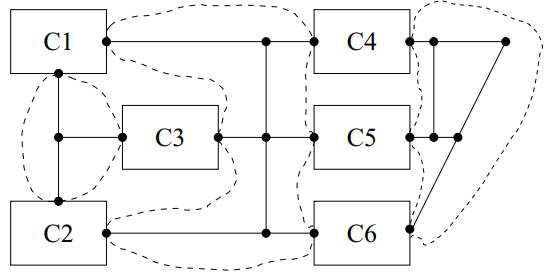
\includegraphics[page=1, width=0.4\textwidth]{images/reoConnector.png}
\caption[]{A system containing compute components $\{C1, C2, ... , C6\}$ with three complex connectors. Each connector is composed of multiple channels, each channel with its own semantics. Image  from~\cite{introReo}.}
\label{fig:reoConnector}
\end{figure}

\section{Effective Language Requirements}
\label{feature}

% it's not much, but it's a starting point
% general to dos: examples that support why do we want these features so we can cite them
% develop each of the features
The community sentiment is that the programmability of distributed and parallel systems is deficient~\cite{coordination,proper,chapel,langNec}. To establish a different perspective, we define requirements we value in a language for well suiting distributed and parallel systems, which allow the description of complex real-world problems. Development of large, reliable applications requires a clear, expressive language. Such systems are more effective when they utilize all the available resources.

\subsection{Reliability}
\label{sec:feature:reliability}
We all desire our written programs to solve the intended problem without any bugs.
This requires that the programming language and the constructs that compose it facilitate this reliability.
M. Lohstroh~\cite{criticalPathReo} claims protocols are hard to understand and that proving their correctness is challenging. Formal verification techniques can check whether the specified requirements are met. A protocol may satisfy safety properties (`something bad will never happen'), or liveness properties (`something good will eventually happen'). 
Even if a protocol is proven to behave as expected, formal methods can not guarantee for this holds once implemented~\cite{criticalPathReo}. The task of proving correctness becomes even more difficult if the utilized tools do not contain the required constructs for isolating protocol code. 

\say{In the absence of proper structures to enforce (or at least encourage) good protocol programming practices, programmers frequently succumb to the temptation of not isolating protocol code.} -- Jongmans et al.~\cite{modularizationReo}.
We need a reliable way to ensure that the implementation phase does not modify the correctness of a protocol. 
This necessitates models which facilitate building correct programs, free of bugs. Smart compilers may understand whether bugs occur and prevent them from unintentionally passing through the compilation phase. Alternatively, the language constructs can lead the programmer to approach the problem in a way that avoids the introduction of errors at all.

\subsection{Productivity}
\label{sec:feature:clarity}
%definition calrity
%readability, clarity, beginner-friendly
Parallel and distributed programming is unlike sequential programming; developers must express complex notions of parallelism, data or task distribution, communication and synchronization. These processes involve a lot of moving parts and can result in highly variable outcomes depending on how computation steps are ultimately interleaved. As such, this work can easily overwhelm a programmer. We wish to provide abstractions for such cases to make these tasks as easy as possible to facilitate productivity \cite{chapel}.

E. A. Lee ~\cite{langNec} and M. Lohstroh ~\cite{criticalPathReo} consider concurrent programs extremely difficult to be understood by humans due to their nontransparent, non-deterministic behaviour; fundamentally, concurrent programs can result in more possible outcomes owing to the additional complexity introduced by arbitrary \textit{interleavings} of actions. Larger programs result in more complex code; in the concurrent and distributed context, this problem is amplified.
B. L. Chamberlain et. al. ~\cite{chapel} state that the gap between the developers that can effectively program parallel machines and sequential ones enlarges with the time.
%example for Distributed too?
To combat this growing divide, programmers need all the help they can get, necessitating a more natural, intuitive way of understanding their programs. A language facilitating clearer, more abstract code also achieves productivity in another sense: non-technical people can reason about the implementation.
%.

In Subsection~\ref{sec:feature:reliability}, we asserted that protocols are difficult to understand and check for correctness. As further transformations of these protocols during implementation only make matters worse, we suggest a need to reduce these transformations by preferring higher-level code, closer to the original protocol.
%%%%%%%%%%%%%%%%%%%%%%%%%%%%%%%%%%%%%%%

\subsection{Expressivity}
\label{sec:feature:expressivity}
A necessary requirement for solving real-world problems is the ability to effectively --and with minimal friction-- express them using the constructs provided by a language. 
In case a language alone does not provide enough powerful constructs to illustrate a given problem, it must inter-operate with libraries or allow for a language extension for a collective effort in illustrating the problem.

Furthermore, considering the already existing systems, migrating to a completely new environment is not always possible as it requires resources and willingness to do so. Many components have been developed without considering their integration in a medium where they must communicate and collaborate with other modules. Thus, the designed model must be able to accommodate such components~\cite{manifold}.

%%%%%%%%%%%%%%%%%%%%%%%%%%%%%%%%%%%%%
\subsection{Performance}
\label{sec:feature:performance}
We wish the performance of our systems to be comparable to the performance achievable with the available languages. A language that systemically inhibits the achievable performance of a distributed system cannot always compensate by providing other desirable features such as reliability.
As such, we require that performance is not lost in the attempt to satisfy other requirements.

% Thus, it is necessary that fulfillment of other requirements does not excessively
% Thus, we require that the previous features do not prevent achieving a good performance. At the same time, we find it acceptable with a small trade off in performance for a high improvement in other features. 

In the long term, we believe higher performance is naturally expected as a large user community brings more support, contribution and improvement to a language.
In the short term, a solution is to offer features at multiple levels, higher-level features for easy programming but not a guaranteed excellent performance and lower-level features for accommodating parts of code which wish to be optimized for performance~\cite{chapel}.
 

\section{Satisfying Requirements}
\label{how}
Significant progress has been made in the development of productive languages for concurrent computing. This section explores the desirable language requirements defined in Section \ref{feature}; examples of available languages are provided, along with insight into how they accomplish these requirements and how they inter-relate.

\subsection{Satisfying Reliability}
\label{sec:how:reliability}
% \comment{
%     Reo
%     Exogenous coordination language: you express the protocol in one place → it's easy to see if you program sticks to it. Facilitated by expressive features of the language
%     Rust
%     Implicit memory management with no runtime cost. Facilitated by expressive features of the language
%     Session types
%     Define the type of a communication channel to reflect protocol → compiler can ensure participants ahere
%     Modeling
%     mCRL2
% }
For a program to be reliable, it should perform its task consistently, as expected. Languages need to facilitate their programmers writing the code they intend to write. This simple goal has implications for a language's comprehensibility both for compilers (so that correctness can be definitively verified or errors identified) and humans (so that programs are written correctly in the first place).

\textbf{Reo}, \textbf{Manifold}, along with other exogenous communication languages provide this property in a way most languages do not: protocol code is located in one place~\cite{proper}. This isolation succeeds in more effectively capturing and preserving the \textit{intent} the programmer has in mind. Focusing on this idea of intent makes the mapping from the abstract algorithm to the Reo implementation easier and require less decision-making for the developer; additionally, it allows the problem to be expressed more coarsely, granting the compiler more freedom to optimize the details of the resulting binary. For example, Reo is able to perform \textit{protocol} optimizations such as merging distinct message channels onto one physical link~\cite{reoLinda}. Traditionally, \textit{actions} are first-class primitives and \textit{interactions} are derived concepts i.e. a message emerges from a \textit{send} and \textit{receive}; this spreads the interaction all over the source code.
Reo leans on the notion of upgrading \textit{interactions} to a first-class primitives instead~\cite{introReo}.

\textbf{Rust} is an imperative systems programming language with neither explicit memory management, nor a garbage collector. Its `ownership system' implements affine types, which requires that all data is associated with precisely one `owner' at a time, but may be `borrowed' (passed by reference) temporarily~\cite{rustSystem}. These borrows are gouverned by rules akin to those for the \textit{readers-writer lock}\footnote{The readers-writer lock is a concurrency mechanism for allowing multiple references without data races.}, requiring that no value is ever aliased and mutable at the same time. An example of the relationship between the ownership system and Rust syntax is given in Listing~\ref{lst:ownership}. This system prevents a program with dangling pointers or race conditions from compiling~\cite{patina}. Along with (optional) run-time array bounds-checking, this provides memory safety~\cite{rustbelt,patina}.
% DUMMY DUMMY DUMMY DUMMY DUMMY DUMMY DUMMY DUMMY DUMMY DUMMY DUMMY DUMMY DUMMY


\begin{listing}[t]
\footnotesize
\begin{minted}[breaklines,mathescape,frame=lines,tabsize=4]{rust}
fn foo(x: Data) { // foo consumes given x
	if bar() {
		let y = &mut x; // x aliased mutibly
	} // y goes out of scope
	baz(&x, &x); // x aliased with read-only refs
	// x references out of scope
} // x is dropped
\end{minted}
\caption{Illustration of the Rust ownership system (implementing affine types). References alias values with pointers until the references go out of scope. A mutable reference may not coexist with any other reference. Owned values that go out of scope are dropped implicitly.}
\label{lst:ownership}
\end{listing}

\textbf{Session types} are another paradigm for guaranteeing adherence to a communication protocol, often possible even at compile-time. In a nutshell, session types allow the programmer to express the type of a \textit{session} (representing a communication link) in a type system similar to that typically used for data types. Participants in the protocol can then only participate if the data they pass in or out is the correct type. Multi-party session types extend this notion to links with an arbitrary number of participants~\cite{sessionMultiparty}. Implementations for the various session type schemes either exist already or have been defined for languages Scribble, Rust, C, Erlang, Go, Java, Python, Scala and more~\cite{sessionRust,sessionHaskell}. Its wide adoption can be largely attributed the broad applicability of the concept. They can be implemented via libraries or natively, and checked statically or dynamically, etc. Consequently, languages without native support can be augmented by the addition of session types in a way that best suits the language.

\begin{listing}[t!]
\footnotesize
\begin{minted}[breaklines,mathescape,frame=lines,tabsize=4]{chapel}
config const m = 1000, alpha = 3.0;

const ProblemSpace = {0..m+1} dmapped Block(..), // allow algorithm to run on multiple locales. If unspecified, the domain maps on one locale only
      SubProblemSpace: subdomain(ProblemSpace) = {1..m}; 

var A, Temp: [ProblemSpace] real; // array of size ProblemSpace with elements of type real

//forall = concurrent alternative of for loop
A = alpha * A; // = forall a in A do alpha * a 
[i in SubProblemSpace] Temp[i] = (A[i-1] + A[i+1])/2; // = forall over SubProblemSpace indices
\end{minted}
\caption{Illustration of Chapel global view syntax. The code runs on multiple locales as the domain map was explicitly specified. The last two lines of code imply concurrent execution, each locale executes the code in parallel.}
\label{lst:globalView}
\end{listing}

Not only do we need the tools to create a reliable system, but we also need to be able to verify that it adheres to the protocol. This requires a good understanding of the execution semantics of our system. Analyzing models of the system's behaviour provides this understanding in a way that can be reproduced and easily communicated to others. However, modeling a complex concurrent system can be a challenging task, as was found by numerous sources ~\cite{modelConcurrentProblems,Fokkink2007ModellingDS, concurrentBMCModel}. The nature of exogenous coordination languages such as \textbf{Manifold} and \textbf{Reo} lends themselves well to graphical representations, making visual modelling of complex behavioral protocols a much easier task. For example, the authors of~\cite{model-reo} present a tool for converting Reo into mCRL2~\cite{mcrl2}. mCRL2 is a specification language that can be used to specify and analyze the behavior of distributed systems in Eclipse~\footnote{The most widely-used Java integrated development environment (IDE).}. Thanks to the user-friendly environment of mCRL2 in the Eclipse Coordination Tools (ECT), the implemented protocols can be visualized, verified and checked for correctness. In addition to validation, model-based checking easily maps to declarative models, reducing the gap between specification and implementation. This benefits developers as it is easier to maintain an overview of the implementation, as well as other non-technical stakeholders as they can more easily understand it.

%%%%%%%%%%%%%%%%%%%%%%%%%%%%%%%%%%%%%%%%%%%%%%%%
\subsection{Satisfying Productivity} \label{how:clarity}
% \comment{
%     Linda → manifold → Reo (graphical declarative langs)
%     They all aim 
%     Chapel
%     Impala
%     Transactional memory
%     how it interoperates with other langs
% }

Programming in a distributed setting is very challenging. It requires programmers to make the considerations inherent to sequential programming, with the added challenges of correct concurrency on top. Overcoming this difficulty requires the language to add minimal friction or risk overwhelming a programmer, leaving them unproductive~\cite{langNec}.

 \textbf{Transactional Memory} was introduced in the early 1990s to facilitate abstracting away from the tedious task of manually achieving mutual exclusion. Instead of locks, transactions allow multiple threads to initiate transactions in memory concurrently, keeping track of all read and write operations performed in the \textit{critical section}. Each thread \textit{commits} its changes when done, after which the transaction is irreversible. A check is first performed to determine if an involved memory location was modified by two threads; if so, the thread \textit{rolls back} the transaction, giving another thread an opportunity to commit~\cite{TMIntroduced}. Transactional memory is still an active area of research. However, the high cost of rollbacks inhibits its adoption as the primary solution to highly-concurrent applications~\cite{TMNotSolution}. Nevertheless, this type of abstraction was greatly appreciated by the development community, which still today utilizes transactional memory for specific purposes. We are still today working with the primitives that transactional memory tried to abstract away from, reflecting the necessity of another replacing language, tool or construct.

Where applicable, nothing achieves conciseness quite like a good abstraction. \textbf{Linda} manages to frame all communication operations in terms of four primitive actions on tuples, all variants of getting and setting tuples to and from a single persistent tuple store in the centralized, virtual shared memory `tuple space'~\cite{linda}. During development, Linda developers need only think in terms of these ubiquitous tuple operations, making it very easy to understand how the problem is being solved. It isn't until performance optimization becomes the priority that programmers have to look past the tuple abstraction. Even then, the compiler will do all the heavy lifting, distributing tuples between machines and optimizing ordering according to how they are accessed.

\textbf{Chapel} is a language that attempts to provide the benefits of a high-level global view approach to distributed programming (comparable to an exogenous coordination language) as well as the performance that sometimes requires fine control. At the higher levels, programs look more like pragma-augmented sequential code (familiar to developers that have worked with an OpenMP library), with specialized concurrent loops containing the data-parallel sections of code. An example of high-level global view Chapel can be seen in Listing~\ref{lst:globalView}. Whenever the higher levels differ from the programmer's needs in terms of data distribution, memory reuse etc., programmers can `dive down' to a lower layer, altering data distribution patterns or employing task parallelism~\cite{chapel}. This approach ensures Chapel code is only ever as complex as it needs to be, and granular details are present only because they represent deviations from the norm. 


% \begin{listing}[t!]
% \footnotesize
% \begin{minted}[breaklines,mathescape,frame=lines,tabsize=4]{chapel}
% config const m = 1000,
%       alpha = 3.0;

% const ProblemSpace = {0..m+1} dmapped Block(..), // allow algorithm to run on multiple locales. If unspecified, the domain maps on one locale only
%       SubProblemSpace: subdomain(ProblemSpace) = {1..m}; 

% var A, Temp: [ProblemSpace] real; // array of size ProblemSpace with elements of type real

% //forall = concurrent alternative of for loop
% A = alpha * A; // = forall a in A do alpha * a 
% [i in SubProblemSpace] Temp[i] = (A[i-1] + A[i+1])/2; // = forall over SubProblemSpace indices
% \end{minted}
% \caption{Illustration of Chapel global view syntax. The code runs on multiple locales as the domain map was explicitly specified. The last two lines of code imply concurrent execution, each locale executes the code in parallel.}
% \label{lst:globalView}
% \end{listing}

\textbf{Rust} offers a similar duality with `unsafe' code blocks. By marking a block with an explicit keyword, some operations that are not checked by Rust's ownership system are permitted~\cite{rustSystem}. This allows a programmer to explicitly manipulate raw pointers or statically type-cast values~\cite{patina}. The Rust community encourages the use of `pure safe rust', with popular libraries touting this safety in their doc pages. Unsafe Rust is used for cases where the compiler cannot be convinced of safety without turning to a sub-optimal formulation. Consider, for example, \textit{hogwild}, where threads write to a shared variable without locking, as the algorithm converges correctly regardless of arbitrary overwrites~\cite{hogwild}. The ownership system would prohibit these unsafe writes, as correctness cannot be inferred by the compiler~\cite{rustlang}.
%%%%%%%%%%%%%%%%%%%%%%%%%%%%%%%%%%%%%%%%%%%%%%%%%%%
\subsection{Satisfying Expressivity}
\label{sec:how:expressivity}

%A very small set of channels, each with very simple behavior, suffices to construct useful Reo connectors with significantly complex behavior. from proper

The architectural expressiveness of \textbf{Reo} make it well-suited for our purpose. The communication topology of components can be naturally established and described~\cite{criticalPathReo} making Reo accessible to developers. Figure~\ref{fig:reoArch} shows an example of an expressive communication model, a point-to-point model. Modifying one of the components make it easy to reason on how it may impact the other components~\cite{introReo}.
\begin{figure}
\centering
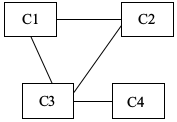
\includegraphics[page=1, width=0.25\textwidth]{images/reoArch.png}
\caption[h]{Architectural expressiveness. Communication pattern of a peer-to-peer model. The effect of modifying or replacing a component can be seen from this model, namely which other components will be affected. Image from~\cite{introReo}.}
\label{fig:reoArch}
\end{figure}
%Reo allows arbitrary user-defined channels as primitives; arbitrary mix of synchrony and asynchrony; and relational constraints between input and output. from proper

A study on the expressive power of Reo and Linda shows that the channel-based coordination model is surely more expressive as it allows mixing synchronous and asynchronous behaviour~\cite{reoLinda}.
For the same reason, Reo is considered more expressive than Manifold which only allows asynchronous behaviour~\cite{criticalPathReo}. 
Furthermore, Reo is more expressive than dataflow models, Kahn networks, synchronous languages, stream processing languages, workflow models and Petri nets~\cite{proper}.


% Chapel
Another prime example of an expressive language is \textbf{Chapel}. The global view programming model together with Chapel's language constructs for achieving data and task parallelism as described in Subsection \ref{how:clarity} represent principles that allow meaningful expression of real-world problems. 

Additionally, Chapel wishes to achieve interoperability with other languages such as C, to accommodate existing components~\cite{chapel}.
The support for calling between Chapel and C was already accomplished. Chapel is able to use external declaration of C concepts, i.e. functions, variables and types~\cite{chapelSite}.
At the time of writing, the interface with  C++, Java, Python, Fortran is in the process of being achieved through Babel, a high-performance language interoperability tool. Babel 2.0 includes an experimental version of Braid, which is an ongoing effort to support, among other languages, Chapel~\cite{babelSite}.

%%%%%%%%%%%%%%%%%%%%%%%%%%%%%%%%%%%%%%%%%%%%%%%%%%%%%
\subsection{Satisfying Performance}
\label{sec:how:performance}
% \comment{
%     Compilers do the dirty work
%     Reo and the sweet graph thingy
%     Rust compile time memory stuff
%     how it interoperates with other langs
% }
 

The ownership system of the \textbf{Rust} programming language, first outlined in Section~\ref{sec:how:reliability} and exemplified in Listing~\ref{lst:ownership}, is a purely compile-time construct. Rust is intended as a systems programming language; this incentivizes strong memory safety, while also necessitating competitive performance. While safe, the use of a garbage collector is prohibitively expensive. Instead, a Rust binary looks much like one created by a C compiler, with explicit allocation and de-allocation. These calls are inserted by the compiler at positions implicit by the structure of the source code~\cite{rustSystem}. Further language-integrations such as string slices allow generically-written iterator code without incurring run-time cost~\cite{slicing,vectorization}. This feature along with powerful and safe abstract macros\footnote{Macros in Rust are not based on string preprocessing. Rather, macros define operations on tokens in subtrees of the abstract syntax tree at compile time.} suit Rust well for the application of writing combinatory parsers for things like VLC Media Player's demuxers~\cite{rustParse,nom}.


% \begin{listing}[t]
% \footnotesize
% \begin{minted}[breaklines,mathescape,frame=lines,tabsize=4]{rust}
% fn foo(x: Data) { // foo consumes given x
% 	if bar() {
% 		let y = &mut x; // x aliased mutibly
% 	} // y goes out of scope
% 	baz(&x, &x); // x aliased with read-only refs
% 	// x references out of scope
% } // x is dropped
% \end{minted}
% \caption{Illustration of the Rust ownership system (implementing affine types). References alias values with pointers until the references go out of scope. A mutable reference may not coexist with any other reference. Owned values that go out of scope are dropped implicitly.}
% \label{lst:ownership}
% \end{listing}

\textbf{Impala} is a domain-specific dialect of Rust that seeks to take all of the syntax and much of the foundations of Rust to GPU programming. As with Rust, Impala leverages a novel, semantic-rich language extension to allow the compiler to optimize code extensively. Impala provides pragma\footnote{Pragmas are instructions in code that typically involve \textit{meta}-programming on other code constructs rather than mapping to anything in the binary; For example, inlining functions.}-like annotations which allow a compiler to evaluate some statements at compile-time, exploding control structures ahead of time; an example is provided in Listing~\ref{lst:partialEval}. Other instances generate code that exhibits `continuation-passing style', chaining functions together by passing subsequent code into functions as call arguments. These optimizations are exploited extensively by various GPU architectures, allowing further coalescing of task granularity for GPU threads. These features allow Impala to compile down to OpenGL and CUDA targets, making it portable while performing competitively~\cite{impala}.

\begin{listing}[t!]
\footnotesize
\begin{minted}[breaklines,mathescape,frame=lines,tabsize=4]{rust}
fn dot(a: &[i32], b: &[i32], n: i32) -> i32 {
    let mut sum = 0;
    for i in range(0, n) {
        sum += a(i) * b(i);
    }
    sum
}

fn main() -> i32 {
    let (a, b) = /* (omitted) */;
    let c = @dot(a, b, 4); // @ marks partial eval.
    
    /*  This generates:
    let mut c = 0;
    c += a(0) * b(0);
    c += a(1) * b(1);
    c += a(2) * b(2);
    c += a(3) * b(3);
	*/
}
\end{minted}
\caption{Example of an annotation in Impala resulting in partial evaluation of a function. Combined with normal compiler optimizations this results efficient GPU code. Source: \url{https://anydsl.github.io/Impala}.}
\label{lst:partialEval}
\end{listing}

\textsc{dream} is an aerodynamics application used to simulate the behaviour of fluids around moving bodies.
During the development, the authors report an extensive comparison between the message passing framework, PVM, and \textbf{Linda}~\cite{pvm, LindaVSMessage}. The evaluation is made on a cluster and both \textit{hardware performance} and \textit{elapsed time} are taken into consideration. The authors report consistent results of Linda outperforming PVM when scaling up the number of nodes and/or workload. This is mainly due to Linda's virtual shared memory system, offering automatic \textit{load balancing} capabilities in the tuple-space. This does not only allow for better scaling, but also requires less effort when developing. The results from the paper when running 9 compute nodes are visualized in Figure \ref{fig:pvmVsLinda}.

\begin{figure}[]
\centering
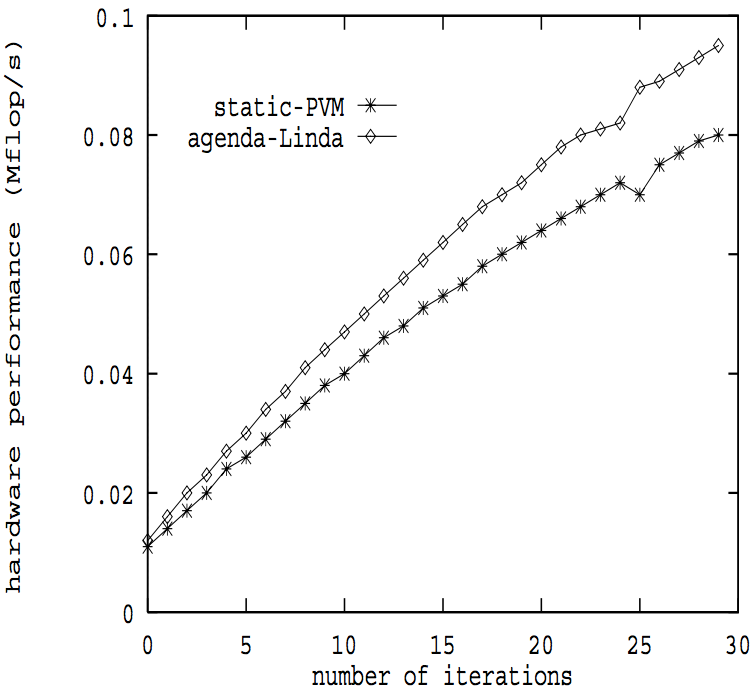
\includegraphics[page=1, width=0.45\textwidth]{images/pvmVsLinda.png}
\caption[]{Hardware performance of Linda and PVM applications for increasing number of time steps in the TDSL phase, using a 9-node multi-computer. Image from~\cite{LindaVSMessage}.}
\label{fig:pvmVsLinda}
\end{figure}

\textbf{Linda} outperforms PVM in scalability and execution speed. Furthermore, the authors stress that Linda was especially useful as `rapid application development platform', significantly decreasing the development time in comparison to PVM. Thanks to Linda's structure, the authors could perform different experiments by altering the coordination, a task which would take much more time in message passing framework due to its fine-grained structure. This case study shows how an abstract coordination language can be well-suited for the development of a complex distributed system containing many different tasks. Stitching components together is typically easier in a language that decouples process coordination and computation, since this provides a more easily maintained overview and more loosely coupled components. This holds also when using different programming languages~\cite{reoLinda}. As a result of their experience, the authors chose to continue to develop their system \textsc{dream}, with the tools offered by the Linda programming environment.

Despite its high-level approach, \textbf{Reo} has been shown to be capable of competing with hand-optimized C code. Reo is able to take the high-level protocol definition and apply \textit{protocol-level optimization} (deduplicating communication links, etc.) during compilation. Even more importantly, Reo is capable of leveraging the \textit{Proto-Runtime-Toolkit} (PRT) for all its granular concurrency primitives. PRT offers control over system resources \textit{without} involvement of the OS scheduler~\cite{proper}; Figure \ref{fig:reoPerf} illustrates this positive result. Arbab et al. argue that many imperative languages cannot hope to meaningfully compile down to PRT the way Reo does, as the languages are too fine-grained for the compilers to be able to effectively map native source code to PRT. PRT is far too platform-specific and low-level for any programmer to interact with productively for any implementation of realistic complexity. They summarize this sentiment in Figure~\ref{fig:actInter}; for the imperative example, the large effort of the programmer is illustrated by the large `distance' from the high-level declarative algorithm to the low-level imperative implementation in a traditional language. The corresponding compiler has little room to apply optimizations as the code it is provided with is already highly specified. By contrast, the Reo-approach affords a smaller step from algorithm to implementation by the programmer, relegating more granular work to the compiler. For this reason, the compiler is at liberty to perform optimizations at the protocol level as well as those used in both cases to make best use of the quirks of the target machine (cache coherence, etc.). Arbab et al. recognize that in both cases optimizations are performed, but in the latter case, they are performed by the less error-prone \textit{compiler} rather than a human~\cite{proper}.

\begin{figure}
\centering
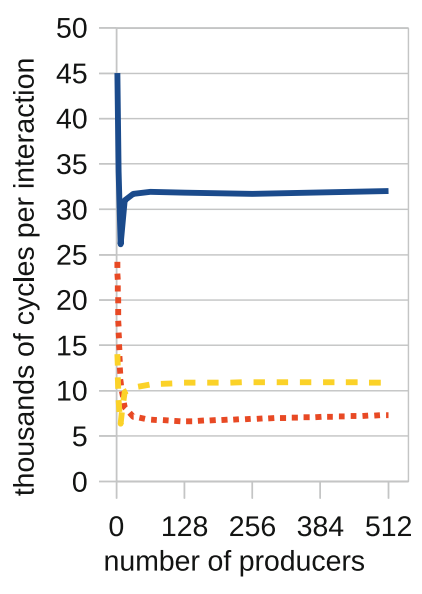
\includegraphics[page=1, width=0.27\textwidth]{images/reoPerf.png}
\caption[]{CPU cycles per interaction for N-Producer-1-Consumer implementation with na\"{i}ve C implementation in solid navy, hand-optimized C implementation in dashed yellow and Reo in dotted red.. Image from~\cite{proper}.}
\label{fig:reoPerf}
\end{figure}


\begin{figure}
\centering
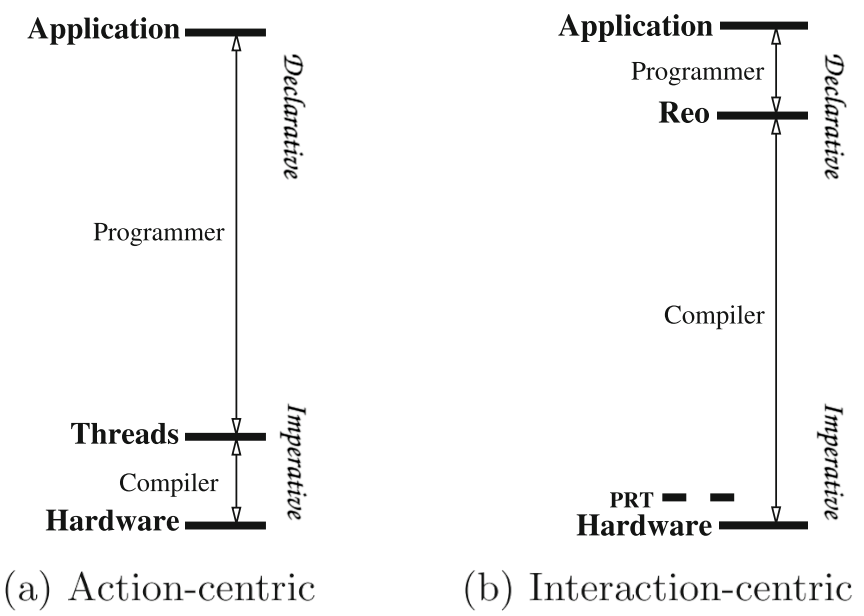
\includegraphics[page=1, width=0.46\textwidth]{images/actInter.png}
\caption[]{Visualization of the transformations necessary from the abstract algrithm to the ultimate imperative machine code for (a) a traditional, imperative language like C (b) Reo. Image from~\cite{proper}.}
\label{fig:actInter}
\end{figure}


% \begin{figure}
% \centering
% 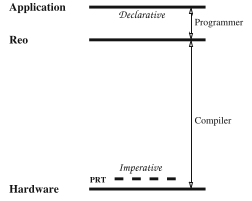
\includegraphics[page=1, width=0.4\textwidth]{images/interaction.png}
% \caption[]{Visualization of the transformations necessary from the abstract algrithm to the ultimate imperative machine code, in this case for Reo. Image from~\cite{proper}.}
% \label{fig:interaction}
% \end{figure}




\section{Trade-offs}
\label{tradeoff}
This section explores the weaknesses of the languages from Section~\ref{how}. We discuss how these weaknesses are currently mitigated and how they might be improved further in the future.


\textbf{Chapel}'s layered approach to the granularity of code, as discussed in \ref{how:clarity}, allows the programmer to gloss over details when a high-level approach is sufficient. Unfortunately, Chapel's high-level `global view' has been found to under-perform when compared to the same algorithm implemented in the lower, `local view'. This is a result of the compiler's shortcoming, and perhaps a mismatch between the expectations of the programmer and the actions of the compiler. With refinement, development of the Chapel language hopes to incrementally close this performance gap~\cite{chapel,globalViewChaphel}.


Coordination languages have shown immense promise, with \textbf{Linda} and \textbf{Reo} both showcasing all of our selected requirements. \textbf{Linda} has been shown to out-perform a message-passing competitor significantly, particularly for larger-scale systems~\cite{LindaVSMessage}; this is explored further in Section~\ref{sec:how:performance}. However, these findings are out of date, while comparisons to more modern competitors are scarce. \textbf{Reo} is a newer language, and it benefits from more up-to-date performance measurements to relevant technologies (such as C with MPI)~\cite{proper}. Overall, it demonstrates competitive performance, as described in Section~\ref{sec:how:performance}. Unfortunately, an experiment found Reo to be between 10\% and 40\% slower in 25\% of cases, suggesting that performance is not guaranteed to consistently exceed that of imperative languages~\cite{proper}. Concerns have also been raised about the \textbf{reliability} of Reo, as the exploration of their formal correctness has not yet been thoroughly proven. This is the case for many languages while still in early development. Owing to its verifiable nature, we believe Reo will overcome this limitation given time to develop.

The ownership system present in \textbf{Rust} and \textbf{Impala} does not incur any run-time performance penalty, as explored in 
\ref{sec:how:performance}. However, memory safety necessitates that the programmer specifies the \textit{lifetimes} of variables in scope in relation to one another~\cite{rustSystem}. In practice, this means code is sometimes peppered by lifetime variables, which leads to a loss of \textbf{clarity} at first glance. The Rust developers have considered this, and have added \textit{lifetime elision rules} that allow the compiler to implicitly infer omitted lifetimes in most cases~\cite{rustlang}. Programmers also experience `fighting with the compiler', attempting to express something not inherently memory-safe (as with the \textit{hogwild} example in Section~\ref{how:clarity}). This can be considered a lack of \textbf{expressiveness} in the language. Fortunately, Rust's \textit{unsafe} language subset is intended for precisely this purpose, ensuring such restrictions in expressivity are more like speed-bumps, and less like road-blocks.

%%%%%%%%%%%%%%%%%%%%%%%%%%%%%%%%%%%%%%%%%%%%%%%%%%%
%\label{sec:tradeoff:general}
A more general problem when programming with high-level tools that abstract away from an underlying low-level implementation, it is desired that the resulting implementation is less complex than if the same task would be solved in this underlying language. This closely relates to the \textit{complexity gap}, stating that there is an arbitrarily large gap between two complexity classes and discussing the bound relating the two~\cite{complexityGap}. In some cases one could argue that a task could be more trivially solved in a low-level language such as C, rather than using a more abstract language or tool, compiling down to a similar code base. Acknowledging that this in some cases can be true~\cite{chapel}; we should not focus on these individual cases but on the bigger picture. In, for example, a declarative system, one can more effectively maintain the separation of semantics and implementation. This implies less implementation complexity for future reference or when adding extra functionality. Also, systems tend to grow in complexity as functionality is added~\cite{coordination}. With this, the complexity gap between the two quickly diminishes, especially when a system scales in a more complex setting, such as parallel and distributed computing. See Section~\ref{how} for more insight into why abstracting away from low-level language is desirable.


\section{Conclusions}
\label{conclusion}
% \comment{
% We have seen examples that work well. We conclude that things are moving in the right direction and that developers should start adopting them, researchers should continue exploring them and students should start learning them
% We admit not all the languages we identified have all the perfect features we are interested in, however, just about all of them are more feature-rich than MPI+C
% }
%Take-home message: if the reader remembers only 1 thing about your work, what should it be?
%Draw conclusions from your work (significance, limitations, learnt)
%In what sense will the world be a better place now that you have solved this problem

% \begin{enumerate}
%     \item We found some strong contenders, many partial successes but Reo stands out as having achieved all 4
%     \item many new langs found they bring new stuff to the table, reliability etc
%     \item performance isn't an issue as much as it used to. in some cases it overachieved, but the issue isnt 100 percent resolved (future work)
%     \item we completely and utterly SMASHED the illusion LOL, already better than C and MPI. hope more attention will cause issues to be resolved faster etc.
% \end{enumerate}


% \comment{Started a new suggestion underneath, but it contains stuff from above}


With parallel and distributed computing systems becoming increasingly mainstream, we need the appropriate programming languages and tools to accommodate for this paradigm shift. Message passing frameworks such as MPI, based on primitives developed decades ago, are the most widely-used solutions for this concurrent context. However, after the examination of several novel programming languages, we argue that modern, high-level languages are just as good, if not better at solving these problems.

We identify and elaborate on four crucial requirements in modern concurrent systems: reliability, productivity, expressivity and performance. Several modern languages make meaningful, innovative contributions in these areas. Reo, in particular, distinguished itself in making significant strides in all requirements at once, while Linda shows excellent scalability in memory management using clever load-balancing. We emphasize the importance of using a tool which can be applied intuitively in a complex setting, maintaining a comprehensible overview of the code and facilitating formal protocol validation. Languages such as Reo, Chapel and Linda accomplish this by abstracting away from low-level details while still providing the necessary expressiveness. This results in developers benefiting from a faster and smoother development process, arriving at a more structured implementation. We observe how high-level languages have begun to close the performance gap with low-level languages. For example, Rust, Impala and Reo achieve strong memory and protocol safety without performance cost by relying on well-defined type systems at compile-time. Furthermore, Reo's nature afforded the Proto-Runtime-Toolkit as a compilation target, resulting in programs that use system resources without OS scheduling overhead, circumstantially out-performing hand-written optimized C-code. We identified several such viable alternatives to established messages passing frameworks.

We encourage developers to not stick to what they know and investigate these high-level programming languages. In many cases, it could result in a maintainable system with better reliability and performance.



\section{Acknowledgments}
Many thanks to Roy Overbeek for his guidance on the topic of coordination languages, particularly in his knowledge of Reo and the research behind it.

\noindent

{\footnotesize \bibliographystyle{acm}
\bibliography{references}}

% \theendnotes
\end{document}
